 \subsection{Constraints}
To ensure an IIR filter stability, the design of the filter adheres to two key constraints identified in \cite{vanwaterschoot2014}. The first constraint mandates that the poles and zeros should be aligned on identical radial lines in z-plane. The second constraint requires that both poles and zeros reside within the unit circle, with zeros positioned between the adjacent poles.

These constraint can be mathematically interpreted in the context of filter design. A zero positioned close to the unit circle, denoted as $z_{i}=$ $r_{i} e^{j \omega_{i}}$, with $r_{i}$ approaching unity, effectively attenuates frequencies in close proximity to $\omega_{i}$. Conversely, a pole is situated on the same radial line, represented as $p_{i}=\alpha r_{i} e^{j \omega_{i}}$, introduces a resonant effect at $\omega_{i}$ that  serves to narrow the notch's bandwidth. 

\subsection{Q Format}\label{q_format}
The Q format is a fixed-point number representation commonly used in DSP to enable efficient arithmetic operations on fractional numbers under limited resources. 

A Q format number is represented by notation $Q_{m.n}$, denoting a fixed-point format with 'm' integer bits and 'n' fractional bits. For instance, the specification Q2.14, describes a signed binary fixed-point number with a 16-bits in total, comprising the sign bit, one bit for the integer part, and 14 bits that are the fraction. Namely, a 16-bit signed, or two's complement, integer, is implicitly multiplied by the scaling factor $2^{-14}$.

While the TMS320C5515 DSP board supports arithmetic in 16-bit and 32-bit fixed-point formats, the constraints of register width invariably impose a ceiling on precision that it is inherently limited to 16-bit precision.

Given the ranges of variables empirically observed in the input signal, the corresponding Q formats that represent these values without overflow and with sufficient precision are as follows:

\begin{itemize}
    \item \textbf{Variable $e$} with range \([-0.7970, 0.6775]\), indicated as a signed short which magnitude never exceed unity, is allocated a 16q15 format.
    \item \textbf{Variable $s$} with range \([-4.7065, 4.7443]\), represented a signed short with absolute values under five, is aptly depicted in a 16q11 format, reserving one bit for the sign and four for the integer.
    \item \textbf{Variable $a$} within \([0.9999, 1.9131]\), exhibiting a positive range with an upper limit below two, is expressed as an unsigned short in 16q15 format.
\end{itemize}

With particular attention to the input frequency response at narrow bands of $400Hz$ and $1200Hz$, the following Q formats were found suitable:

\begin{itemize}
    \item \textbf{Variable $\rho$} consistently remains below one and is non-negative, warranting a 16q16 format, fully fractional, represented as an unsigned short.
    \item \textbf{Variable $\mu$}, as predetermined, is in a 16q15 format.
    \item \textbf{Variable $\lambda$} presents a non-negative range capped at maximum one, adhering to a 16q15 format.
\end{itemize}

\subsection{Adaptive Notch Filter Implementation}
The implementation of the Adaptive Notch Filter (ANF) using the Least Mean Squares (LMS) algorithm is encapsulated within a single function. This function is responsible for dynamically adjusting the filter coefficients to minimize the error between the desired and actual filter outputs.

\subsubsection{Function Description}
The ANF function takes as input the current sample of the signal, a pointer to a state buffer that retains the last three samples, a pointer to the adaptive filter coefficient, a pointer to the current and asymptotic values of the bandwidth adjustment parameter $\rho$, and a pointer to the current index in the circular buffer. It returns the filtered signal sample.

% Derived from \autoref{q_format}, the filter is designated with input parameters as outline in \autoref{fig:input_params}.

% \begin{figure}
%     \centering
%     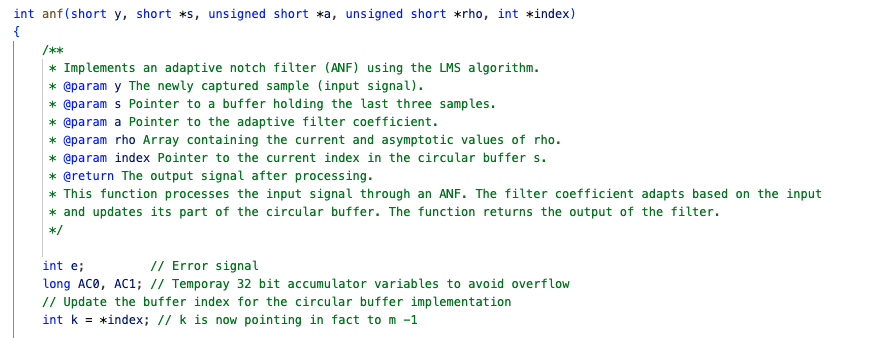
\includegraphics[width=0.7\linewidth]{images/c_code_input_param.png}
%     \caption{Input parameters type of ANF function in C}
%     \label{fig:input_params}
% \end{figure}

Derived from \autoref{q_format}, the filter is designated with input parameters as below:
\begin{lstlisting}[language=C, basicstyle=\small]
int anf(short y, short *s, unsigned short *a, unsigned short *rho, int *index)
{
    /**
     * Implements an adaptive notch filter (ANF) using the LMS algorithm.
     * @param y The newly captured sample (input signal).
     * @param s Pointer to a buffer holding the last three samples.
     * @param a Pointer to the adaptive filter coefficient.
     * @param rho Array containing the current and asymptotic values of rho.
     * @param index Pointer to the current index in the circular buffer s.
     * @return The output signal after processing.
     */
     ......
}
\end{lstlisting}

The data type $short$ of the newly captured sample $y$ is identical to the one of samples stored in the data buffer $s$. $Index$ pointer having $int$ data type to allow for positive and negative indexing in the circular buffer. In the perspective of filter, $a$, the adaptive coefficient, and $\rho$, ratio for adjusting bandwidth configuration embedded within $pole$ and $zero$, are of type $unsigned\ short$.  

\subsubsection{Algorithm Steps}
The function performs the following steps in the ANF-LMS algorithm:

\begin{enumerate}
    \item It calculates the new value of $\rho(m)$, which is a weighted average of its previous value and the asymptotic value, using the coefficients $\lambda$ and $1 - \lambda$. This step ensures that the filter's bandwidth can adapt over time.
    
    \item The state buffer $s$ is updated to reflect the newest sample. This buffer operates in a circular fashion, using the modulo operation to maintain a fixed-size history of the samples.
    
    \item The error signal $e(m)$ is computed, incorporated with latest computed $s(m)$, representing the difference between the desired signal and the filter's output. This error is then used to update the adaptive filter coefficient.
    
    \item Finally, the adaptive filter coefficient $a(m)$ is adjusted based on the error signal and the learning rate $\mu$. This coefficient determines the notch's depth and width, allowing the filter to suppress the undesired frequencies effectively.
\end{enumerate}

The program makes use of 32-bit accumulators to prevent overflow during intermediate calculations. The function also includes a check to constrain the adaptive filter coefficient that $\left\lvert (a(m)) \right\rvert < 2 $, ensuring the stability of the filter.

\subsubsection{Q-format alignment} 
While variables consists of varied Q-format, Q-format alignment prior to blocks of additions and multiplications are required. In our DSP implementation, Q format alignment is exemplified especially during the computation of signal processing terms. Consider the calculating of first term of $s(m)$, which involves the product of $rho(m)$, $a(m-1)$, and $s(m-1)$. Here $\rho[0]$ represented in $Q16$ format, is multiplied by $a[k]$ in $16q15$ format, yielding an intermediate result in $32q31$. This results is then rounded and normalized back to $16q15$ format by right-shifting the accumulator $ACO$, which aligns the Q format for the subsequent multiplication with $s[k]$ in $16q11$ format. The final shift of $ACO$ by $A-Q-FORMAT$ bits ensures that the result is in the desired $16q11$ format, ready to be integrated into $s(m)$.

\begin{lstlisting}[language=C, basicstyle=\small]
// Calculate the first term of s[m]: rho(m) * a(m - 1) * s(m - 1) with k = (m - 1)
AC0 = (long)rho[0] * a[k]; // 16q16 * 16q15 = 32q31
AC0 += 0x4000;             // Add half (since we are shifting 15 bits) to round
AC0 >>= RHO_Q_FORMAT;      // Now AC0 is 32q15
AC0 *= s[k];               // 32q15 * 16q11 (assuming s is in q15 format) = 32q26
AC0 >>= A_Q_FORMAT;        // Normalize to 32q11
\end{lstlisting}

\subsubsection{Circular Buffer Mechanism}
The circular buffer is a key component for implementing the IIR filter, as it allows for efficient memory usage by reusing buffer positions rather than sequentially updating each indexed content, storing the history of samples. The index and k management ensures that the oldest sample is overwritten with the newest one, and that when the function call is finished, the index points to the latest processed index which will be used as the $m-1$ in the next function call.

\subsubsection{Coefficient Adaptation}
The adaptive nature of the filter is realized through the constant update of the coefficient $a(m)$, which is influenced by the error signal and she historical samples. The LMS algorithm ensures that the coefficient converges to a value that minimizes the error signal over time, thereby nullifying the effect of the undesired frequencies.

\subsubsection{Stability and Convergence}
To maintain the stability of the filter, the function includes bounds checking for the coefficient values to not exceed $0x7FFF$, which is two in $16q15$ foramt. Additionally, the shift operations are carefully managed to maintain the fixed-point precision defined by the Q format.

\subsection{Input Parameter Storage register}
The capability of TMS320C5515 registers were studied for effective variables memory manipulation, which is especially critical in assembly programming. As the variables pass from the main script consist of one $short \ y$ where the remaining parameters are of pointers to variables such as $short*$ or $unsigned short*$, registers hypothesized to stored/point to the inputs params are correspondingly $T0$, $AR0$, $AR1$, $AR2$, $AR3$, and return $short\ e$ again in $T0$. The auxilary register were employed given that the specific input parameters are of pointer type that requires manipulation in address phase, which often combined with 23-bit $XARx$ for address and data operations.



